\section{Fin Design}

\subsection{Trade Study}

Multiple attitude control methods were considered for the GLD design including jet tabs, jet vanes, and external fins. An overview of each of these concepts is shown in Figures \ref{fig:atitudectrl_conc}.

\begin{figure}[H]
    \centering
    \begin{subfigure}[b]{0.3\textwidth}
        \centering
        
\includegraphics[height=1.2in]{AtitudeControl_Figures/fins.png}
        \caption{Fins}
    \end{subfigure}
    ~
    \begin{subfigure}[b]{0.3\textwidth}
        \centering
        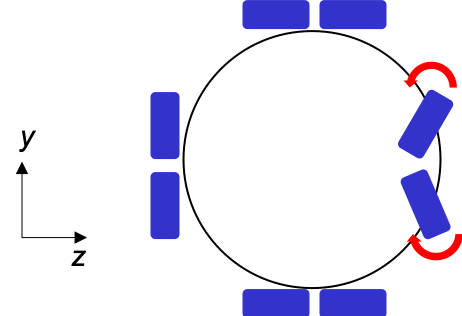
\includegraphics[height=1.2in]{AtitudeControl_Figures/tabs.png}
        \caption{Jet Tabs}
    \end{subfigure}
    ~
    \begin{subfigure}[b]{0.3\textwidth}
        \centering
        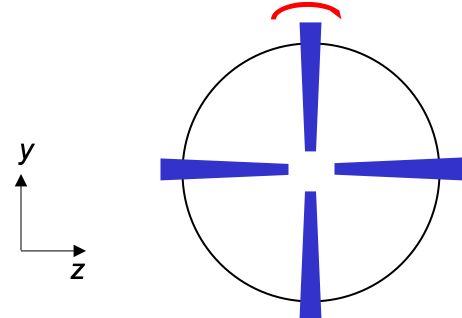
\includegraphics[height=1.2in]{AtitudeControl_Figures/vanes.png}
        \caption{Jet Vanes}
    \end{subfigure}
    \caption{Overview of attitude control system concepts \label{fig:atitudectrl_conc}}
\end{figure}

Missiles that utilize fins for attitude control are typically comprised a set of static fins and a set of maneuverable fins. The static fins are designed to help control the location of the vehicles center of pressure over its operational envelope while the maneuverable fins provide the control torque about the center of gravity. The fin control scheme can be configured such that the maneuverable fins are located forward of the vehicle center of gravity or such that the maneuverable fins are located aft-ward of the center of gravity. Tail control provides better control authority at high angles of attack in comparison to canard control and typically is used in long range applications. Conversely, canard (forward) control is better for low angle of attack and short range applications. Since the SFRJ design will be performing aggressive maneuvers and is designed to maximize range, only tail control was considered when trading fins against other concepts.

The jet tab concept operates by obstructing the nozzle exhaust flow with blunt bodies which alters the effective thrust vector angle of the vehicle. This concept is attractive due to its simple and low power construction and because it does not generate any performance loss for the vehicle when it is not being used. However, thrust losses of are predicted to be a maximum of approximately 5\% for our application \cite{eatough1977} with limited control authority especially in the roll axis when compared to the fin design.

Jet vanes present a hybrid approach between the jet tab and fin designs. Maneuverable fins are located in the nozzle exhaust stream to control the thrust vector. This approach provides limited advantages over the jet tab and fin methods due to the large performance losses that it induces, its high power requirements, and complexity to design. Due to these disqualifying limitations, the jet vane concept was not considered during final attitude control method selection.

Power, complexity of design, control authority, performance loss, and mass were the prime factors considered in the final design selection. To accurately compare the jet tab and tail fin approaches, a preliminary design was generated for each method. CAD renders of the two designs are displayed in Figure \ref{fig:atitudectrl_prel} below. The fin design consists of four fins with a angle of attack range from -5$^\circ$ to 5$^\circ$. Each fin is driven by a single electrical actuator with a 1.575 inch moment arm. The jet tab design is comprised of four sets of two jet tabs. The tabs in a set rotate counter to each other and are driving by two DC motors on a single gear train. The performance of the fins was characterized with linear supersonic theory while the jet tab design was characterized using empirical data from previous designs \cite{eatough1977}. When these two preliminary designs were compared, it was determined that while the fin design requires twice as much electrical power as the jet tabs, it also provides better control authority, was lower mass, and required a simpler mechanism design. It is for these reasons that the tail fin control scheme was selected for the GLD design.

\begin{figure}[H]
    \centering
    \begin{subfigure}[b]{0.45\textwidth}
        \centering
        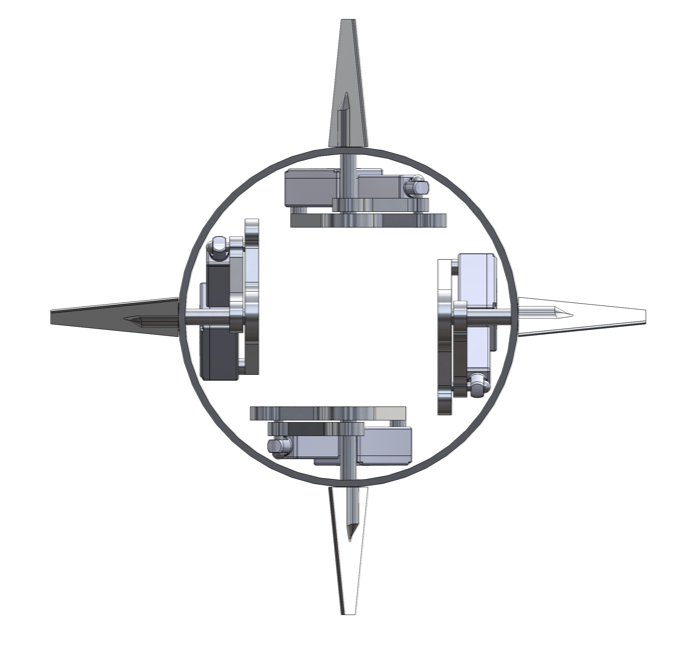
\includegraphics[width=3.0in]{AtitudeControl_Figures/fin_design.png}
        \caption{Tail Fins}
    \end{subfigure}
    ~
    \begin{subfigure}[b]{0.45\textwidth}
        \centering
        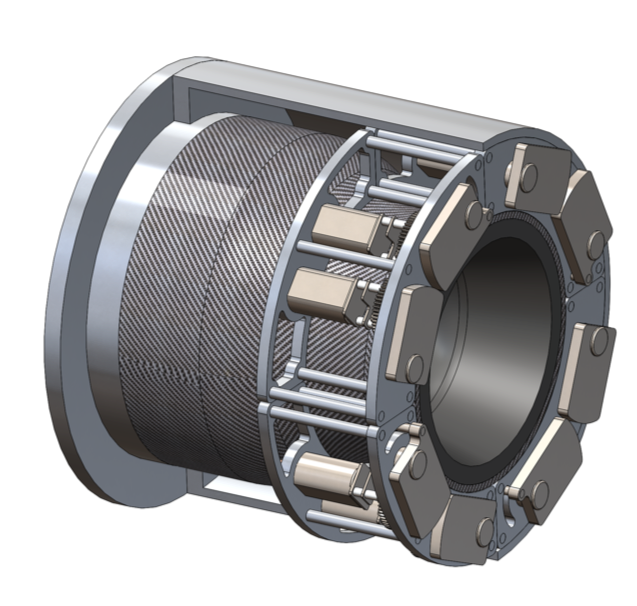
\includegraphics[width=2.75in]{AtitudeControl_Figures/tab_design.png}
        \caption{Jet Tabs}
    \end{subfigure}
    \caption{Preliminary Attitude Control Concepts \label{fig:atitudectrl_prel}}
\end{figure}

\pagebreak

\subsection{Design Overview}

\begin{multicols}{2}

    \begin{wrapfigure}{R}{0.5\textwidth}
        \begin{center}
        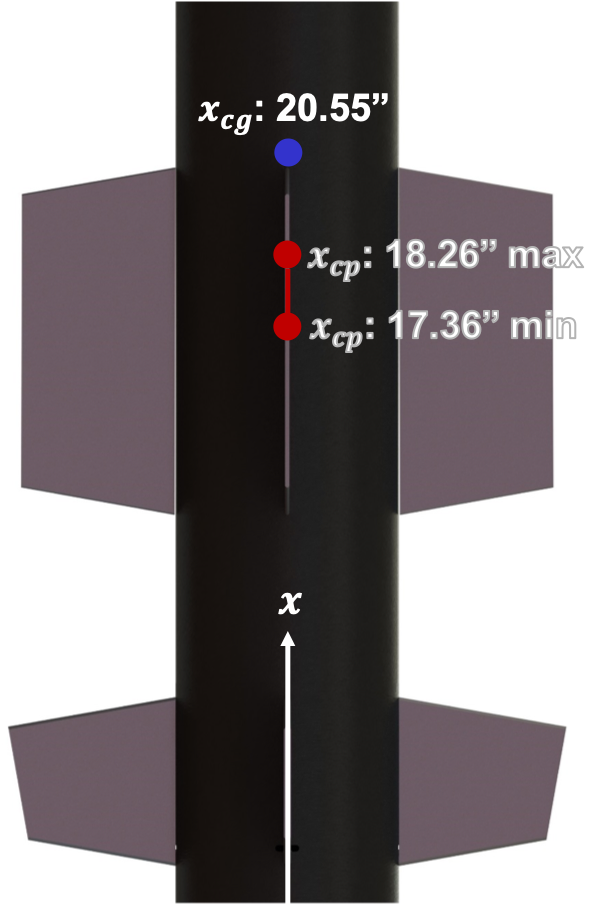
\includegraphics[width=\linewidth]{AtitudeControl_Figures/fin_int_design.png}
        \end{center}
        \caption{Integrated Fin Design \label{fig:fin_int_design}}
    \end{wrapfigure}
\end{mui

\subsection{Analysis \& Sizing}

\subsection{Future Work}